\documentclass[aps,pra,twocolumn,superscriptaddress,nofootinbib,10pt]{revtex4-2}

\usepackage{amsmath,amssymb,amsfonts,bm}
\usepackage{booktabs}
\usepackage{tikz}
\usepackage[colorlinks=true,linkcolor=blue,citecolor=blue,urlcolor=blue]{hyperref}

\begin{document}

\title{Sub-Harmonic Injection Locking and Gyrotropic Parity Symmetry Breaking\\
in a Low-Pressure Argon Standing-Wave RF Cavity Processor}

\author{Justin D. Grimm}
\altaffiliation{ORCID: 0009-0000-5299-0243}
\affiliation{Independent Dandelion Substrate Research Group,
Gurley, Alabama 35748, USA}

\date{November 17, 2026}

\begin{abstract}
We formulate the electrodynamic field theory, radioisotopic timing protocol,
and hardware-software control architecture (v1.1.0) for a continuous-wave
balanced-ternary ($\{-1, 0, +1\}$) standing-wave processor operating inside a
copper-lined spherical cavity of inner radius $a = 0.1431\text{ m}$ filled
with low-pressure Argon ($P = 1.067\text{ kPa}$). Centering electron energy
near the $0.23\text{ eV}$ Ramsauer-Townsend scattering minimum suppresses
momentum-transfer damping ($\nu_m / \omega_0 = 0.0153$) on the fundamental
$\text{TM}_{101}$ eigenmode at $f_0 = 915.0\text{ MHz}$ ($Q_L = 1850$). A
phase-coherent third-harmonic pump at $3f_0 = 2.745\text{ GHz}$ establishes
three symmetric $120^\circ$ phase basins above the ternary Landauer erasure
floor $k_B T_g \ln 3$. To eliminate achiral domain-wall pinning ($D_3$
stagnation) on a frustrated $N = 13$ equatorial probe ring, longitudinal
beta helicity from an exempt $37.0\text{ kBq}$ $^{60}\text{Co}$ source paired
with a sub-cyclotron $28.0\text{ mT}$ axial Helmholtz field induces an
off-diagonal gyrotropic permittivity and a $10.50^\circ$ non-reciprocal
Sakaguchi phase lag ($D_3 \to C_3$), while modulo-13 decimated $37.0\text{ kBq}$
$^{241}\text{Am}$ alpha tracks provide a crystal-free $104.0\text{ Hz}$
Erlang-13 frame clock.
\end{abstract}

\maketitle

\section{Introduction and Falsification Contract}

Conventional complementary metal-oxide-semiconductor (CMOS) logic computes by
repeatedly charging and discharging nodal capacitances across discrete binary
thresholds, dissipating orders of magnitude more heat than the thermodynamic
minimum identified by Landauer~\cite{Landauer1961} and verified experimentally
by B\'{e}rut \textit{et al.}~\cite{Berut2012}. Oscillator-based Ising and Potts
machines~\cite{Traversa2015,Wang2019} reduce switching overhead by encoding
discrete variables into continuous phase degrees of freedom under sub-harmonic
injection locking (SHIL). However, on geometrically frustrated odd-ring graphs
such as $N = 13$, standard symmetric phase coupling preserves dihedral
reflection symmetry ($D_3 \cong \mathbb{Z}_3 \rtimes \mathbb{Z}_2$): clockwise
and counter-clockwise phase kinks possess degenerate Helmholtz free energy and
mutually pin in metastable achiral traps.

Here we resolve achiral pinning at the physical substrate level by coupling
three mechanisms inside a single partial-vacuum spherical cavity: (i) low-loss
standing-wave storage inside Argon's Ramsauer-Townsend elastic minimum,
(ii) nuclear-paced Erlang-$k$ frame timing and localized Bragg-peak refractive
perturbations via degraded $^{241}\text{Am}$ alpha tracks, and (iii) explicit
parity symmetry breaking ($D_3 \to C_3$) driven by weak-interaction beta
helicity~\cite{Wu1957,Wauters2010} in a sub-resonant axial magnetic guide field,
yielding physical realization of the non-reciprocal Kuramoto-Sakaguchi phase
lag~\cite{Sakaguchi1986}.

\vspace{4pt}
\noindent\fbox{\parbox{0.96\columnwidth}{%
\textbf{Experimental Falsification Protocol (v1.1.0):}
\begin{enumerate}
\item \textbf{Chiral Unpinning ($D_3 \to C_3$):} At $B_0 = 0.0\text{ mT}$
($\alpha_\chi = 0^\circ$), frustrated $N = 13$ anneals must exhibit bimodal
winding $\langle W \rangle \approx 0$. Energizing $B_0 = 28.0\text{ mT}$
($\alpha_\chi = 10.50^\circ$) must lock steady-state winding onto $W = +1$
across $\ge 95\%$ of trials; failure falsifies gyrotropic parity coupling.
\item \textbf{Erlang-13 Nuclear Regularity:} Across $10^4$ frames at effective
rate $A_{\text{eff}} = 1352\text{ s}^{-1}$, inter-frame intervals must obey
$\mu_\tau = 9.615\text{ ms}$ ($104.0\text{ Hz}$) and
$\sigma_\tau / \mu_\tau = 1/\sqrt{13} = 0.2774 \pm 0.015$ with zero crystal
harmonic spurs.
\item \textbf{Sub-Breakdown \& Zero-Tick Safety Closure:} Continuous
$915.0\text{ MHz}$ drive ($0.50\text{ W}$, $8.13\text{ kV/m}$) must remain
$\ge 9.4\text{ dB}$ below Argon self-breakdown ($24.0\text{ kV/m}$), and any
reflected VSWR surge above $0.50\text{ V}$ must mute RF/HV rails in zero state
ticks.
\end{enumerate}}}
\vspace{4pt}

\section{Bounded Cavity Electrodynamics}

Let $\Omega \subset \mathbb{R}^3$ denote a copper-lined non-magnetic sphere of
inner radius $a$ operated over strictly bounded causal epochs
$t \in [t_m, t_{m+1}]$ with $0 < t_{m+1} - t_m < \tau_{\max}$. The cavity
electric field $\bm{E}(\bm{r}, t)$ obeys the curl-curl wave equation:
\begin{equation}
\nabla \times (\nabla \times \bm{E})
+ \frac{1}{c^2}\frac{\partial^2}{\partial t^2}
  \Big(\bar{\bar{\bm{\varepsilon}}}_r(\bm{r}, t)\bm{E}\Big)
+ \mu_0 \frac{\partial \bm{J}_{\text{cond}}}{\partial t}
= -\mu_0 \frac{\partial \bm{J}_{\text{pump}}}{\partial t}.
\label{eq:wave}
\end{equation}
Matching the lowest spherical transverse-magnetic root $u_{11} = k_0 a = 2.7437$
to the $f_0 = 915.0\text{ MHz}$ industrial-scientific-medical (ISM) band
($\omega_0 = 5.749 \times 10^9\text{ rad/s}$) fixes the inner radius at
$a = 0.1431\text{ m}$ ($12.27\text{ L}$) and the cold-plasma cutoff density at
$n_c = \varepsilon_0 m_e \omega_0^2 / e^2 = 1.04 \times 10^{16}\text{ m}^{-3}$.

At static Argon pressure $P = 1.067\text{ kPa}$ ($8.0\text{ Torr}$, neutral
density $n_g = 2.58 \times 10^{23}\text{ m}^{-3}$ at $T_g = 300\text{ K}$),
quantum $s$-wave interference produces the Ramsauer-Townsend cross-section
minimum ($\sigma_{\text{RT}} \approx 1.2 \times 10^{-21}\text{ m}^2$) near
electron energy $E_e \approx 0.23\text{ eV}$, holding collisional damping to
$\nu_m / \omega_0 = 0.0153$ and preserving a loaded quality factor
$Q_L = 1850$ ($\tau_{\text{cav}} = 2Q_L/\omega_0 = 0.64\text{ }\mu\text{s}$).
Four primary ports arranged at the tetrahedral angle
$\theta_{\text{tet}} = \arccos(-1/3) = 109.47^\circ$ establish a 3D frustrated
nodal core at $\bm{r} = \bm{0}$, sampled by $N = 13$ equatorial pickup loops.
To prevent vacuum O-ring seams from bisecting the equatorial probes, the vessel
parting collar is placed at polar angle $\theta_{\text{split}} = 72.00^\circ$
($z = +0.04422\text{ m}$), leaving all 13 pickups in a single monolithic bowl.

\begin{figure}[t]
\centering
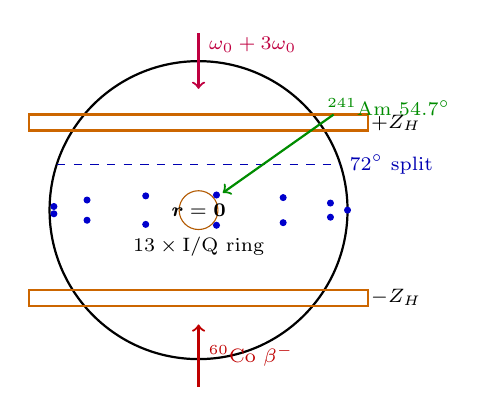
\begin{tikzpicture}[scale=0.88, every node/.style={font=\scriptsize}]
  \draw[thick] (0,0) circle (2.15cm);
  \draw[dashed, blue!70!black] (-2.04,0.66) -- (2.04,0.66)
    node[right] {$72^\circ$ split};
  \draw[thick, orange!80!black] (-2.45,1.15) rectangle (2.45,1.38);
  \draw[thick, orange!80!black] (-2.45,-1.38) rectangle (2.45,-1.15);
  \node at (2.85,1.26) {$+Z_H$};
  \node at (2.85,-1.26) {$-Z_H$};
  \draw[->, thick, red!75!black] (0,-2.55) -- (0,-1.65)
    node[midway,right] {$^{60}\text{Co }\beta^-$};
  \draw[->, thick, green!55!black] (1.95,1.38) -- (0.35,0.25)
    node[pos=0.15,above right] {$^{241}\text{Am }54.7^\circ$};
  \draw[->, thick, purple] (0,2.55) -- (0,1.75)
    node[pos=0.2,right] {$\omega_0 + 3\omega_0$};
  \draw[thin, orange!70!black] (0,0) circle (0.28cm);
  \foreach \k in {0,...,12} {
    \filldraw[blue!80!black] ({2.15*cos(\k*27.692)}, {0.22*sin(\k*27.692)})
      circle (1.2pt);
  }
  \node at (0,-0.52) {$13\times\text{I/Q ring}$};
  \node at (0,0) {$\bm{r}=\bm{0}$};
\end{tikzpicture}
\caption{Cross-section of the $a = 0.1431\text{ m}$ Argon cavity showing the
$72.0^\circ$ dome collar, $\pm Z_H$ Helmholtz coils ($28.0\text{ mT}$),
magic-angle $^{241}\text{Am}$ port ($54.74^\circ$), axial $^{60}\text{Co}$ port,
and monolithic 13-port equatorial homodyne ring.}
\label{fig:cavity}
\end{figure}

\section{Radioisotopic Bragg Perturbation and Gyrotropic Parity Bias}

Mounting an exempt $37.0\text{ kBq}$ $^{241}\text{Am}$ source behind a
$12\text{ }\mu\text{m}$ polymer energy degrader at the magic angle
$\theta_m = \arccos(1/\sqrt{3}) = 54.74^\circ$ sets the second Legendre
polynomial $P_2(\cos\theta_m) = 0$ and steps exit alpha energy down to
$E_{\text{exit}} = 0.95\text{ MeV}$, parking the terminal Bragg peak inside
$\bm{r} = \bm{0}$ at $1.067\text{ kPa}$. With Argon ionization potential
$W_{\text{Ar}} = 26.4\text{ eV}$ and ballasted sub-breakdown Townsend gain
$M = 1.0 \times 10^4$, each alpha injects $\Delta N_e \approx 3.6 \times 10^8$
electrons ($\Delta n_e \approx 0.035\,n_c$), deflecting local refractive index
by $3.5\%$. Decimating a guard PIN diode modulo $k = 13$ converts Poissonian
decays into an Erlang-13 frame clock:
\begin{equation}
f_{13}(\tau; A_{\text{eff}})
= \frac{A_{\text{eff}}^{13}\tau^{12}e^{-A_{\text{eff}}\tau}}{12!},
\qquad \mu_\tau = \frac{13}{A_{\text{eff}}} = 9.615\text{ ms}.
\label{eq:erlang}
\end{equation}

To lift $D_3$ reflection degeneracy, an axial $37.0\text{ kBq}$ $^{60}\text{Co}$
Gamow-Teller $\beta^-$ source ($\langle E_\beta \rangle = 96.5\text{ keV}$,
intrinsic longitudinal helicity $\mathcal{H} = -v_e/c = -0.548$, empirical
asymmetry $\tilde{A}_{\text{exp}} = -1.014$~\cite{Wu1957,Wauters2010}) injects
left-handed tracks along an axial Helmholtz guide field $B_0 = 28.0\text{ mT}$
($\omega_{ce}/\omega_0 = 0.8565$, safely below exact $32.69\text{ mT}$ electron
cyclotron resonance). The cold-plasma permittivity acquires an antisymmetric
off-diagonal gyrotropic component $\varepsilon_g$:
\begin{equation}
\bar{\bar{\bm{\varepsilon}}}_r =
\begin{pmatrix}
\varepsilon_\perp & -i\varepsilon_g & 0 \\
i\varepsilon_g & \varepsilon_\perp & 0 \\
0 & 0 & \varepsilon_\parallel
\end{pmatrix}, \quad
\varepsilon_g = \frac{\omega_{ce}}{\omega_0}
\frac{\omega_p^2}{\omega_0^2 - \omega_{ce}^2 + \nu_m^2}.
\label{eq:gyro}
\end{equation}
Projecting $\bar{\bar{\bm{\varepsilon}}}_r - \bm{I}$ onto the 13 equatorial
eigenmodes under third-harmonic SHIL ($2.745\text{ GHz}$) yields the coupled
Chiral Kuramoto-Sakaguchi-SHIL equations:
\begin{equation}
\frac{\mathrm{d}\phi_i}{\mathrm{d}t}
= \Delta\omega_i + \Omega_\chi - K_s(t)\sin(3\phi_i)
+ \sum_{j=1}^{13} |J_{ij}|\sin(\phi_j - \phi_i - \alpha_\chi)
+ \xi_{\text{iso},i}(t),
\label{eq:ckss}
\end{equation}
where modal filling $\Gamma_{\text{fill}} = 0.201$ plus the $+1.27\%$
quadrupolar offset locks $\alpha_\chi = \arctan(\Gamma_{\text{fill}}
\omega_{ce}/\omega_0) + \delta_{\chi,E2} = 0.1833\text{ rad}$ ($10.50^\circ$).
Phase attractors $\phi_i^* \in \{-2\pi/3, 0, +2\pi/3\}$ map bijectively onto
balanced trits $s_i = \mathrm{round}(3\phi_i^*/2\pi) \in \{-1, 0, +1\}$ above
the ternary Landauer bound $W_{\min} \ge k_B T_g \ln 3 \approx 1.0986\,k_B T_g$
per reset trit~\cite{Landauer1961,GrimmKembali2026}.

\begin{table}[b]
\caption{Benchtop Cavity, Nuclear, and RF Link Budget (v1.1.0).}
\label{tab:budget}
\begin{ruledtabular}
\begin{tabular}{lllr}
Subsystem & Parameter & SI Value & Margin / Role \\
\hline
Cavity $\text{TM}_{101}$ & Inner radius $a$ & $0.1431\text{ m}$ & $915.0\text{ MHz}$ \\
Argon fill & Pressure $P$ & $1.067\text{ kPa}$ & $Q_L = 1850$ \\
Tetrahedral RF & Continuous drive & $0.50\text{ W}$ & $9.4\text{ dB}$ sub-arc \\
SHIL $3\omega_0$ & Harmonic pump & $0.25\text{ W}$ & $2.745\text{ GHz}$ \\
Helmholtz $B_0$ & Axial DC field & $28.0\text{ mT}$ & $\alpha_\chi = 10.50^\circ$ \\
$^{241}\text{Am}$ / $^{60}\text{Co}$ & Exempt sources & $37.0\text{ kBq}$ ea. & $104.0\text{ Hz}$ frame \\
13x Homodyne & Baseband CNR & $123.9\text{ dB}$ & $0.04^\circ$ rms jitter \\
\end{tabular}
\end{ruledtabular}
\end{table}

\section{Closed-Loop CAD, Homodyne PCB, and FPGA Arbitration}

Table~\ref{tab:budget} summarizes the hardware link budget. To eliminate local
oscillator (LO) self-mixing DC drift in the 13 `ADL5380` homodyne receivers, the
`iCE40HX8K-CT256` arbiter inserts a $50.0\text{ }\mu\text{s}$ RF-muted,
LO-active dark calibration slot on every Erlang-13 strobe before classifying
each channel via the division-free integer bound $\sqrt{3} \approx 28378/16384$
and computing phase via a shared 14-stage `Q3.13` CORDIC engine ($69.4\text{ }\mu\text{s}$
total latency). Six auxiliary `AD7606C-16` channels monitor forward/reflected
RF power, SHIL envelope, Townsend current, $B_0$, and vessel temperature,
enforcing zero-tick fail-closed muting (`Code 253`) ahead of `64-byte` SPI DMA
transfers~\cite{GrimmKembali2026,GrimmWaveguide2026}.

\textbf{Open Boundary ($N > 13$):} Extending the equatorial pickup ring to prime
cardinalities $N \in \{17, 19, 37\}$ on higher-order $\text{TM}_{m10}$ whispers
enables multi-word Potts partitioning within the same vacuum envelope; we
leave experimental characterization of multi-bolus Townsend space-charge
saturation at $N \ge 19$ to subsequent wet-cavity trials.

\begin{thebibliography}{9}
\bibitem{Landauer1961}
R. Landauer, IBM J. Res. Dev. \textbf{5}, 183 (1961),
\href{https://doi.org/10.1147/rd.53.0183}{doi:10.1147/rd.53.0183}.

\bibitem{Berut2012}
A. B\'{e}rut, A. Arakelyan, A. Petrosyan, S. Ciliberto, R. Dillenschneider,
and E. Lutz, Nature \textbf{483}, 187 (2012),
\href{https://doi.org/10.1038/nature10872}{doi:10.1038/nature10872}.

\bibitem{Traversa2015}
F. L. Traversa and M. Di Ventra, Chaos \textbf{25}, 103106 (2015),
\href{https://doi.org/10.1063/1.4931570}{doi:10.1063/1.4931570}.

\bibitem{Wang2019}
T. Wang and J. Roychowdhury, in \textit{Unconventional Computation and Natural
Computation}, LNCS Vol. 11493 (Springer, 2019), pp. 232--256,
\href{https://doi.org/10.1007/978-3-030-19311-9_19}{doi:10.1007/978-3-030-19311-9\_19}.

\bibitem{Wu1957}
C.-S. Wu, E. Ambler, R. W. Hayward, D. D. Hoppes, and R. P. Hudson,
Phys. Rev. \textbf{105}, 1413 (1957),
\href{https://doi.org/10.1103/PhysRev.105.1413}{doi:10.1103/PhysRev.105.1413}.

\bibitem{Wauters2010}
F. Wauters \textit{et al.}, Phys. Rev. C \textbf{82}, 055502 (2010),
\href{https://doi.org/10.1103/PhysRevC.82.055502}{doi:10.1103/PhysRevC.82.055502}.

\bibitem{Sakaguchi1986}
H. Sakaguchi and Y. Kuramoto, Prog. Theor. Phys. \textbf{76}, 576 (1986),
\href{https://doi.org/10.1143/PTP.76.576}{doi:10.1143/PTP.76.576}.

\bibitem{GrimmKembali2026}
J. D. Grimm, \textit{Gemini-Carbon-Kembali 64-Byte Zero-Copy Triadic
Microkernel} (Zenodo, 2026),
\href{https://doi.org/10.5281/zenodo.24288018}{doi:10.5281/zenodo.24288018}.

\bibitem{GrimmWaveguide2026}
J. D. Grimm, \textit{Raychaudhuri Focusing and Chiral Soliton Phase-Locking on
Coupled Dispersive Waveguides} (Zenodo, 2026),
\href{https://doi.org/10.5281/zenodo.24211350}{doi:10.5281/zenodo.24211350}.
\end{thebibliography}

\end{document}
